%##################################################################################################

The tasks embedded within the \texttt{survive} category of our benchmark aim to analyze an AI agent's ability to ensure its own survival, adeptness in combat scenarios, and its capability to interact with the environment in order to meet basic needs. Survival, being a core aspect of Minecraft gameplay, necessitates an intricate balance of offensive, defensive, and sustenance-related actions. This category is structured to ensure a thorough evaluation of these skills. 

\begin{figure*}[h]
%\framebox[4.0in]{$\;$}
\begin{center}
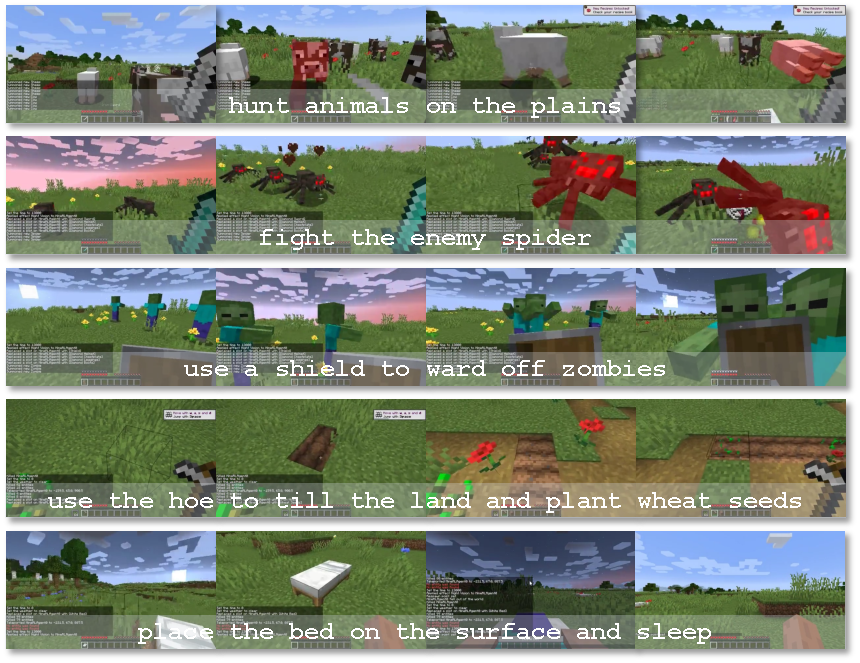
\includegraphics[scale = 0.9]{figures/benchmark_survive.pdf}
\end{center}
\caption{Examples of tasks in \texttt{survive} category. }
\end{figure*}

\definecolor{codeblue}{rgb}{0.25,0.5,0.5}
\definecolor{codekw}{rgb}{0.85, 0.18, 0.50}
\definecolor{keywordgreen}{rgb}{0,0.6,0}
\lstset{
  backgroundcolor=\color{gray!10},
  basicstyle=\fontsize{8pt}{9pt}\ttfamily\selectfont,
  columns=fullflexible,
  breaklines=true,
  captionpos=b,
  commentstyle=\fontsize{7.5pt}{7.5pt}\color{codeblue},
  keywords = {Task, Description, Time, Evaluation, Precondition, SkillAssessed}, 
  keywordstyle = {\textbf},
  caption={The environment configuration and evaluation metric for \texttt{survive} series tasks. },
  label={lst:minecraft_deps_prompt}
}
\begin{lstlisting} % [language=python]  

Task: hunt animals
Description: Hunt animals on the plains. 
Precondition: Spawn the player in the plains biome with an iron sword in the main hand. Spawn 5 sheep and 5 cows near the player's position. 
SkillAssessed: Predator instincts, combat efficiency, and sustenance acquisition.
Evaluation: Ignore animals and run away. < Hurt animals. < Kill animals. 

Task: combat enemies
Description: Fight the enemy spider. 
Precondition: Spawn the player in the plains biome with a diamond sword in its main hand and a suite of diamond equipment. Spawn 3 spiders in front of the player. 
SkillAssessed: Self-defense, offensive combat strategy, and equipment utilization.
Evaluation: Ignore spiders and run away. < Hurt spiders. < Kill spiders. 

Task: use shield
Description: Use a shield to ward off zombies. 
Precondition: Spawn the player in the plains biome with a shield in its main hand and a suite of diamond equipment. Spawn 3 zombies in front of the player. 
SkillAssessed: Defensive tactics, tool application in combat, and strategic protection. 
Evaluation: Ignore zombies and run away. < Use the shield to protect itself. 

Task: plant wheats
Description: Use an iron_hoe to till the land and then plant wheat seeds. 
Precondition: Spawn the player in the plains biome with an iron hoe in its main hand, and a stack of wheat seeds in the off hand. 
SkillAssessed: Land cultivation, planting proficiency, and sustainable resource creation.
Evaluation: Just run away. < Till the land. < Plant the wheats. 

Task: sleep on the bed
Description: Place the bed on the surface and sleep. 
Precondition: Spawn the player in the plains biome with a white bed in its main hand. 
SkillAssessed: Self-preservation, understanding of day-night cycle implications, and use of utilities for rest. 
Evaluation: Just run away. < Place the bed on the surface. < Sleep on the bed. 

\end{lstlisting}


